\documentclass[11pt]{book}
\usepackage[utf8]{inputenc}
\usepackage{adjustbox}
\usepackage{ltablex}
\usepackage{rotating}


%captioning
\usepackage[format=hang,justification=raggedright,  font={small,singlespacing}, labelfont={small,sf,bf}]{caption}
%Spacing
\usepackage{setspace}
\setstretch{1.15}


% Font:
\renewcommand{\rmdefault}{bch}
\renewcommand{\sfdefault}{phv}


% page margins 
\usepackage[paperheight=9in,paperwidth=7in,top=1in,bottom=1in,right=1in,left=1in]{geometry}
%\usepackage[cam,letter,center]{crop}

% lists:
%\usepackage{enumitem}
% tables
\usepackage{booktabs}
\usepackage{array}

\newcolumntype{P}[1]{>{\centering\arraybackslash}p{#1}}
\newcolumntype{M}[1]{>{\centering\arraybackslash}m{#1}}

% headers and footers
\usepackage{fancyhdr}
\usepackage{emptypage} % removes headers and footers from empty pages

%%%% Section and chapter titles
\usepackage{titling}

%%%%%Headings and chapter titles
\usepackage{titlesec}
%Make "Chapter 1" all caps
\renewcommand{\chaptername}{CHAPTER}

%%%%%%%%%%%%%%%%%%%%%%%%%%%%%%%

% addtional packages for the book
%\usepackage{chapterbib}
\usepackage{makeidx}

% these come from the full latex experience through pandoc

\usepackage{amssymb,amsmath}
\usepackage{ifxetex,ifluatex}
\ifnum 0\ifxetex 1\fi\ifluatex 1\fi=0 % if pdftex
  \usepackage[T1]{fontenc}
%  \usepackage[utf8]{inputenc}
  \usepackage{textcomp} % provides euro and other symbols
\else % if luatex or xelatex
  \usepackage{unicode-math}
  \defaultfontfeatures{Scale=MatchLowercase}
  \defaultfontfeatures[\rmfamily]{Ligatures=TeX,Scale=1}
\fi
% use upquote if available, for straight quotes in verbatim environments
\IfFileExists{upquote.sty}{\usepackage{upquote}}{}
\IfFileExists{microtype.sty}{% use microtype if available
  \usepackage[]{microtype}
  \UseMicrotypeSet[protrusion]{basicmath} % disable protrusion for tt fonts
}{}
\makeatletter
\@ifundefined{KOMAClassName}{% if non-KOMA class
  \IfFileExists{parskip.sty}{%
    \usepackage{parskip}
  }{% else
    \setlength{\parindent}{0pt}
    \setlength{\parskip}{6pt plus 2pt minus 1pt}}
}{% if KOMA class
  \KOMAoptions{parskip=half}}
\makeatother
\usepackage{xcolor}
\IfFileExists{xurl.sty}{\usepackage{xurl}}{} % add URL line breaks if available
\IfFileExists{bookmark.sty}{\usepackage{bookmark}}{\usepackage{hyperref}}
\hypersetup{
  pdftitle={Handbook on Using Administrative Data for Research and Evidence-based Policy},
  pdfauthor={Shawn Cole, Iqbal Dhaliwal, Anja Sautmann, Lars Vilhuber},
  pdfborder={0 0 0},
  breaklinks=true}
\urlstyle{same}  % don't use monospace font for urls
\usepackage{longtable}
%\usepackage{booktabs}
% Allow footnotes in longtable head/foot
\IfFileExists{footnotehyper.sty}{\usepackage{footnotehyper}}{\usepackage{footnote}}
\makesavenoteenv{longtable}
\usepackage{graphicx,grffile}
\makeatletter
\def\maxwidth{\ifdim\Gin@nat@width>\linewidth\linewidth\else\Gin@nat@width\fi}
\def\maxheight{\ifdim\Gin@nat@height>\textheight\textheight\else\Gin@nat@height\fi}
\makeatother
% Scale images if necessary, so that they will not overflow the page
% margins by default, and it is still possible to overwrite the defaults
% using explicit options in \includegraphics[width, height, ...]{}
\setkeys{Gin}{width=\maxwidth,height=\maxheight,keepaspectratio}
\setlength{\emergencystretch}{3em}  % prevent overfull lines
\providecommand{\tightlist}{%
  \setlength{\itemsep}{0pt}\setlength{\parskip}{0pt}}
\setcounter{secnumdepth}{5}
% Redefines (sub)paragraphs to behave more like sections
\ifx\paragraph\undefined\else
  \let\oldparagraph\paragraph
  \renewcommand{\paragraph}[1]{\oldparagraph{#1}\mbox{}}
\fi
\ifx\subparagraph\undefined\else
  \let\oldsubparagraph\subparagraph
  \renewcommand{\subparagraph}[1]{\oldsubparagraph{#1}\mbox{}}
\fi

% set default figure placement to htbp
\makeatletter
\def\fps@figure{htbp}
\makeatother

% addtional packages for the book
%\usepackage{chapterbib}
\usepackage[sectionbib,globalcitecopy]{bibunits}
%\usepackage{makeidx}
\usepackage{setspace}
\usepackage{ragged2e}

\usepackage{comment}

\excludecomment{invisible}
% for now - must be included later
\excludecomment{bbox}
\usepackage{booktabs}
\usepackage{longtable}
\usepackage{array}
\usepackage{multirow}
\usepackage{wrapfig}
\usepackage{float}
\usepackage{colortbl}
\usepackage{pdflscape}
\usepackage{tabu}
\usepackage{threeparttable}
\usepackage{threeparttablex}
\usepackage[normalem]{ulem}
\usepackage{makecell}
\usepackage{xcolor}
\usepackage[]{natbib}
\setcitestyle{square}


%
% Workaround
%
\newcommand{\BeginKnitrBlock}[1]{}
\newcommand{\EndKnitrBlock}[1]{}

%
%  automatically add \putbib at end of each chapter

%\ifx\putbib\undefined\else
%    \let\oldchapter\chapter
%    \renewcommand{\chapter}{%
%    \putbib
%    \oldchapter
%  }
%\fi

% 
% Change name of bibliography

\renewcommand{\bibname}{References} % used for non-pandoc compile only

%%%%% bib
\setlength{\bibsep}{0.0pt}
\setlength{\bibhang}{6pt}

\renewcommand{\bibpreamble}{\footnotesize} 
\renewcommand{\bibname}{References in Chapter \thechapter}

%%%%%%%%%%%%%%%%%%%%%%%%%%%

%\setuphead[chapter][align={flushleft, nothyphenated, verytolerant}]

%%%%%Format chapter titles on chapter title pages
\titleformat{\chapter}[display]
  {\Large\sffamily}{\chaptertitlename\ \thechapter}{20pt}{\Huge\bfseries}
\titlespacing*{\chapter}{0pt}{0pt}{40pt}
%%%%%Set heading styles
\titleformat*{\section}{\LARGE\sffamily\bfseries\parindent0pt}
\titleformat*{\subsection}{\Large\sffamily\bfseries}
\titleformat*{\subsubsection}{\large\sffamily\bfseries}
%\renewcommand{\maketitlehooka}{\rmfamily}


%%%%%% Setting headers and footers 
% use after geometry to get right size
\pagestyle{fancy}
\fancyhf{}% Clear header/footer

%Headers:
\makeatletter
\fancyhead[RO]{\sffamily \scriptsize Using Administrative Data for Research and Evidence-Based Policy}
\fancyhead[LO]{ }
\fancyhead[LE]{\sffamily \scriptsize \if@mainmatter CHAPTER \thechapter\fi}
\makeatother
\renewcommand{\chaptermark}[1]{\markboth{#1}{}}

%Footers: 
\makeatletter
\renewcommand{\pagenumbering}[1]{\gdef\thepage{\csname
@#1\endcsname\c@page}}
\makeatother
\fancyfoot{} % clear all footer fields
\fancyfoot[LE,RO]{\small \thepage}
\fancyfoot[LO,CE]{}
\fancyfoot[CO,RE]{}
\renewcommand{\headrulewidth}{0.0pt}

%Make chapter title pages have the same page numbers as the rest:
\fancypagestyle{plain}{% % <-- this is new
  \fancyhf{} 
  \fancyfoot[LE,RO]{\small \thepage} % same placement as with page style "fancy"
  \renewcommand{\headrulewidth}{0pt}}

%%%%%% Title page:
% Formatting the title of the book to flush left
%\pretitle{ \begin{flushleft}\LARGE\sffamily  }
%\posttitle{ \par \end{flushleft} \vskip 2em}

% Formatting the author list

\preauthor{ }
\DeclareRobustCommand{\authorthing}
{\begin{flushleft}\Large
    \begin{tabular}{l}
    %\setlength{\tabcolsep}{1pt}
    Shawn Cole \\ Iqbal Dhaliwal \\ Anja Sautmann \\ Lars Vilhuber 
\end{tabular}

\end{flushleft}
}
\postauthor{}

%%%%%Title here
% Title page
\pretitle{ \begin{flushleft}\LARGE\sffamily  }

\title{ \Large \uppercase{Handbook on} \\\Huge\bfseries {Using Administrative Data \\ for Research and \\ Evidence-based Policy}}
\posttitle{ \par \end{flushleft} \vskip 2em} 

\author{\sffamily \Large \authorthing}
\date{ }


%%%%% Chapter titles with authors in ToC and chapter 
\makeatletter

\newcommand{\chapterauthor}[1]{\authortoc{#1}\printchapterauthor{#1}}

\newcommand{\printchapterauthor}[1]{%
    {\parindent0pt\vspace*{-35pt}%
    \linespread{2}\large\sffamily #1%
    \par\nobreak\vspace*{35pt}}
    \@afterheading%
}
\newcommand{\authortoc}[1]{%
    \addtocontents{toc}{\vskip-10pt}%
    \addtocontents{toc}{%
    \protect\contentsline{chapter}%
    {\parindent0pt\hskip1.5em \mdseries\protect\rmfamily #1}{}{}}
    \addtocontents{toc}{\vskip2pt}%
}
\makeatother

\setlength{\parindent}{0cm}
\setlength{\parskip}{.2cm plus 1mm minus 1mm}


%%%%% TOC
\usepackage{tocloft}
\renewcommand{\cfttoctitlefont}{\sffamily\huge\bfseries}
\renewcommand{\cftchapfont}{\rmfamily \bfseries}
\renewcommand{\cftchappagefont}{\normalfont \small}
%\renewcommand{\cftchapdotsep}{\cftdotsep} 
%\renewcommand{\cftpartleader}{\cftdotfill{}} % for parts

%this keeps the toc from adding extra stuff (subsections)
\setcounter{tocdepth}{0}
\renewcommand{\chaptermark}[1]{%
  \ifnum\value{chapter}>0
    \markboth{Chapter \thechapter{}: #1}{}%
  \else
    \markboth{#1}{}%
  \fi}


%%%%%%%%%%%%%%%%%%%%%%%%%%%%%%%%%%%%%%%%%%%%%%%%%%%%%%%%%%%%%%%%%%%%%%%%%%%%
% Document start
\begin{document}

\bibliographyunit[\chapter]
\defaultbibliographystyle{aea-mod}
\defaultbibliography{packages.bib,ideahandbook.bib}

\frontmatter
\pagenumbering{roman}

\newpage\null\thispagestyle{empty} 
\newpage

 % Title page rendering
\maketitle

\newpage\null\thispagestyle{empty}
\newpage

% TOC
\tableofcontents 


\newpage
\pagestyle{fancy}

\cleardoublepage

\phantomsection
\addcontentsline{toc}{chapter}{About the Editors}

\section*{About the Editors}\label{about-the-editors}

\subsection*{Shawn Cole}\label{shawn-cole}

\href{https://www.hbs.edu/faculty/Pages/profile.aspx?facId=340064}{Shawn
Cole} is the John G McLean Professor of Business Administration at
Harvard Business School. Shawn is a Co-Chair of J-PAL's Innovations in
Data and Experiments for Action Initiative (IDEA). His research examines
agriculture, corporate finance, banking, and consumer finance in
developing countries. He has conducted randomized evaluations in
education, financial literacy, agricultural risk management, and ICT for
agriculture. He received a Ph.D.~in economics from the Massachusetts
Institute of Technology in 2005, where he was an NSF and Javits Fellow,
and an A.B. in Economics and German Literature from Cornell University.

\subsection*{Iqbal Dhaliwal}\label{iqbal-dhaliwal}

\href{https://www.povertyactionlab.org/person/dhaliwal}{Iqbal Dhaliwal}
is the Global Executive Director of J-PAL and co-chair of IDEA. He works
with the Board of Directors to develop J-PAL's strategic vision, with
leadership of the seven regional offices to coordinate J-PAL's worldwide
research, policy outreach, capacity building, and operations, and with
funding partners to secure resources for J-PAL worldwide. He has setup
many partnerships for J-PAL with data providers and implementing
partners. He is a co-PI on a very large randomized evaluation in India
that used both survey data and large admin datasets to help a state
government reduce health care absenteeism. Iqbal has a deep appreciation
of the concerns and constraints of data providers in governments as he
began his career as a member of the Indian Administrative Service (IAS)
formulating policy and implementing programs across many assignments.
Later as a Director in an economic consulting firm in Chicago, he
analyzed numerous very large data sets to provide critical insights to
private sector clients in manufacturing, health, banking and automotive
sectors. He has a BA in economics from the University of Delhi, an MA in
economics from the Delhi School of Economics, and an MPA in
international development from Princeton University.

\subsection*{Anja Sautmann}\label{anja-sautmann}

\href{https://www.worldbank.org/en/about/people/a/anja-sautmann}{Anja
Sautmann} is a Research Economist in the World Bank's Development
Research Group (Human Development Team). She is interested in how
households and individuals make decisions, from healthcare for children
to daily consumption to marriage, and how incentives and individual
behavior shape optimal policy design. Before joining the World Bank,
Anja was an Assistant Professor at Brown University (2010-2017) and the
Director of Research, Education, and Training at the Abdul Latif Jameel
Poverty Action Lab at MIT (2017-2020) and Director of IDEA. She received
her Ph.D.~in Economics from New York University and her diploma in
Economics from Ludwig Maximilians Universität in Munich, Germany. She is
an affiliate of the CESifo research network.

\hypertarget{lars-vilhuber}{%
\subsection*{Lars Vilhuber}\label{lars-vilhuber}}
\addcontentsline{toc}{subsection}{Lars Vilhuber}

\href{https://www.vilhuber.com/lars/}{Lars Vilhuber} is the Executive
Director of the Labor Dynamics Institute at Cornell University, and a
faculty member in Cornell University's Economics Department. He is also
the American Economic Association's Data Editor. Lars is a Co-Chair of
IDEA. His research interests relate to the dynamics of the labor market.
He also has extensive experience in the application of
privacy-preserving publication and access to restricted data. He is
chair of the scientific committee of the French restricted-access system
\href{https://casd.eu}{CASD}, member of the governing board of the
Canadian Research Data Centre Network (\href{https://crdcn.org}{CRDCN}),
and incoming chair of the American Statistical Association`s
\href{https://community.amstat.org/cpc/home}{Committee on Privacy and
Confidentiality}. Lars has an undergraduate degree in Economics from
Universität Bonn and a Ph.D.~in Economics from Université de Montréal.

\section*{About J-PAL}\label{about-j-pal}
\phantomsection
\addcontentsline{toc}{chapter}{About J-PAL}

The Abdul Latif Jameel Poverty Action Lab (J-PAL) is a global research
center working to reduce poverty by ensuring that policy is informed by
scientific evidence. Anchored by a network of more than 225 affiliated
professors at universities around the world, J-PAL draws on results from
randomized impact evaluations to answer critical questions in the fight
against poverty. We build partnerships with governments, NGOs, donors,
and others to share this knowledge, scale up effective programs, and
advance evidence-informed decision-making. J-PAL was launched at the
Massachusetts Institute of Technology in 2003 and has regional centers
in Africa, Europe, Latin America \& the Caribbean, the Middle East \&
North Africa, North America, South Asia, and Southeast Asia.


% Foreword

% \hypertarget{about}{%
%\chapter*{About Us}\label{about}}
%\addcontentsline{toc}{chapter}{About Us}



\mainmatter
\setcounter{page}{1}

% Part 1


% Testing chapters
% this will eventually be replace by files for each chapter

%\include{Introduction.tex}
%\include{Chapter1.tex}

\chapter[Increasing Access to Administrative Data: Why and How?]{Increasing Access to \\ Administrative Data: \\ Why and How?}

\authortoc{Shawn Cole, Iqbal Dhaliwal, Anja Sautmann, Lars Vilhuber}
\printchapterauthor
{    \begin{tabular}{l}
    Shawn Cole, Harvard Business School \\
    Iqbal Dhaliwal, Abdul Latif Jameel Poverty Action Lab \\ 
    Anja Sautmann, World Bank \\
    Lars Vilhuber, Cornell University
\end{tabular}
}
\hrulefill


\section{The Potential of Administrative Data for Research and Policymaking}

Over the course of our careers, we, the editors of this Handbook, have been witness to extraordinary changes in economics and economic research. One of them has been the rise of research in applied microeconomics and development economics that focuses on working closely with policymaking bodies and creating an evidence base for better social programming. Two key factors have contributed to this trend: increased availability of new data sources, and the rapid growth in the use of experiments (randomized control trials or randomized evaluations) in the social sciences. These developments have enabled many new avenues of research, such as how behavioral factors affect optimal policy design, how to credibly evaluate long-run effects of landmark social programs, or how to make changes to these programs informed by a better understanding of the levers of impact. In the process, they have dramatically improved the quality and breadth of evidence used to inform policy.

Yet it is also our experience that this type of research is in many cases conducted by carrying out complex, time-consuming, and costly original data collection: for example, the large-scale surveys that accompany many randomized control trials typically consume a large share of the financial and staff resources devoted to the research project overall. A lack of relevant, reliable, and comprehensive data that researchers can access has been a limiting factor for new studies and consequently the spread of evidence-informed policy.

At the same time, there are a wide variety of data sets already in existence, such as census records, banking data, employment information, or GPS records, which could dramatically reduce the cost and complexity of policy-relevant research – including randomized control trials – and speed up the formation of an evidence base for policymaking. Administrative data, sometimes referred to as organic data (Groves 2011) because they are generated as part of normal business processes, often contain comprehensive, objective data about large populations of interest. Decision-makers at firms and in government are already using such data to better understand problems and issues of populations of interest, and based on such evidence-based analytics, new policies are implemented or new questions are defined.

\begin{figure}[t!]
\caption{Time Trends in the Use of Administrative Data for Empirical
Research. Source: Chetty (2012). Used by permission.}
\centering
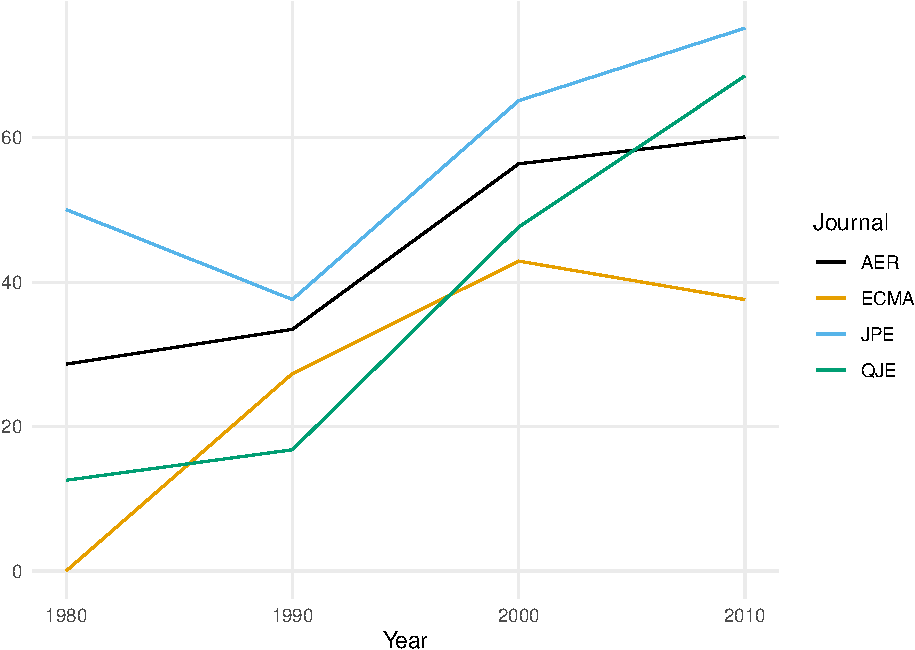
\includegraphics{figures/introchetty-1.pdf}
\rule{1\textwidth}{0.3pt} 
\end{figure}


\begin{figure}[t!]

\centering
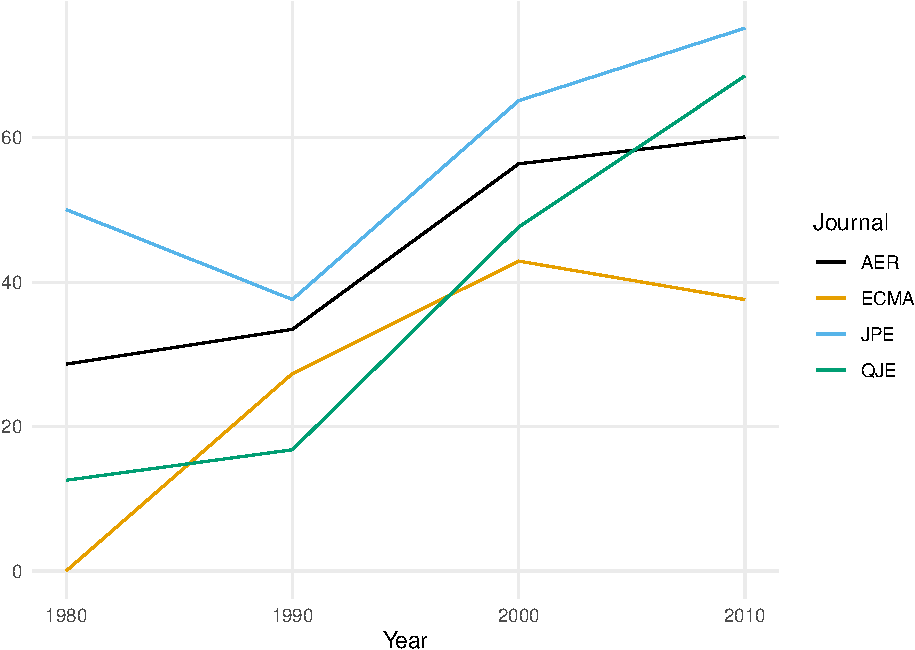
\includegraphics{figures/introchetty-1.pdf}
\caption{Time Trends in the Use of Administrative Data for Empirical
Research. Source: Chetty (2012). Used by permission.}
\rule{1\textwidth}{0.3pt} 
\end{figure}

Beyond these uses, carefully designed systematic research with administrative data, often partnering academic researchers with firms and governments, may carry out analyses, conduct experiments, and develop and field supplemental surveys to test specific mechanisms or hypotheses. This type of innovative research could dramatically expand the types of insights gained from the data. An increasing fraction of published papers in economics uses administrative data (see Figure 1.1, Chetty (2012)). However, researcher access to administrative data sets remains difficult and idiosyncratic (Card et al. 2010). This Handbook is motivated by our view that easier access and an increased use of administrative data sets by researchers could dramatically improve the quantity and quality of available evidence on social programs and policies.
\begin{figure}[t!]
\centering
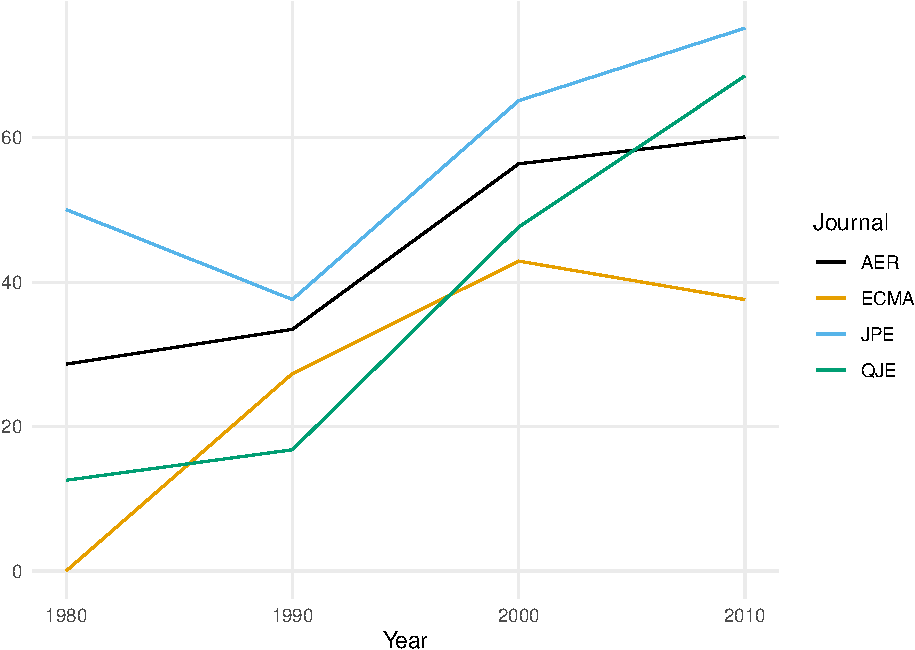
\includegraphics{figures/introchetty-1.pdf}
\caption{Time Trends in the Use of Administrative Data for Empirical
Research. Source: Chetty (2012). Used by permission.}
\end{figure}
Beyond these uses, carefully designed systematic research with administrative data, often partnering academic researchers with firms and governments, may carry out analyses, conduct experiments, and develop and field supplemental surveys to test specific mechanisms or hypotheses. This type of innovative research could dramatically expand the types of insights gained from the data. An increasing fraction of published papers in economics uses administrative data (see Figure 1.1, Chetty (2012)). However, researcher access to administrative data sets remains difficult and idiosyncratic (Card et al. 2010). This Handbook is motivated by our view that easier access and an increased use of administrative data sets by researchers could dramatically improve the quantity and quality of available evidence on social programs and policies.


\newpage
\section{Table example}
\begin{sidewaystable}
%\makebox[\textwidth][c]{
\fontsize{7.5}{10}\selectfont
\begin{tabular}[t]{>{\raggedright\arraybackslash}p{12em}>{\raggedright\arraybackslash}p{8em}>{\raggedright\arraybackslash}p{20em}>{\raggedright\arraybackslash}p{24em}}
\toprule
Case Study & Type of Data Provider & Data Intermediary/Data Holder & Highlight\\
\midrule
Aurora Health Care (AHC, ch.\ 11) & Private company & Data is transferred directly to researchers at MIT and J-PAL & Researcher team helped a private firm think through data protection and cleaning to enable a randomized control trial measuring sensitive health outcomes.\\
City of Cape Town (CCT, ch.\ 13) & City government & Researchers access a server owned by the City to download data & A new data policy led to a productive cooperation between the City and academic researchers to create systematic data access.\\
Development Impact Evaluation, World Bank Group (DIME, ch.\ 14) & Variety of public and private partners & Data is transferred directly to researchers at DIME & DIME's development economists and analysts apply their research expertise and best practices in partnerships with many different administrative data providers.\\
Institute for Employment Research (RDC-IAB, ch.\ 7) & National government agency & RDC-IAB and research data centers at universities provide access to computers that hold the data & A clear legal mandate allows RDC-IAB to distribute German labor market data through a network of remote access points  at national and international research institutions.\\
International Monetary Fund (IMF, ch.\ 15) & Variety of international government partners & Data is held by national governments or transferred directly to researchers at the IMF & As part of its mandate, the IMF helps governments overhaul their tax systems and conduct research on the tax data.\\
\addlinespace
Government of Indonesia (GoI, ch.\ 16) & National government & Data is held by government agencies and transferred directly to researchers & A long-term research partnership enabled multiple nationally representative experiments to improve the targeting of social programs.\\
New Brunswick Institute for Data, Research, and Training (NB-IRDT, ch.\ 9) & Provincial government social protection agencies & Research center at  U.\ of New Brunswick (public) holds and provides data for download to affiliated faculty & A relatively new partnership that has seen rapid expansion in the data that it makes available to researchers, with specific legal mandates for data access and sharing,\\
Ohio Longitudinal Data Archive (OLDA, ch.\ 8) & State agencies & Research center at Ohio State U.\ (public) holds and provides access to the data to approved users & A long-running and successful administrative data partnership that started in 2007. In the last 5 years, 28 published studies have used data accessed through OLDA.\\
Private Capital Research Institute (PCRI, ch.\ 10) & Private firms and publicly available data & An independent, faculty-led non-profit (PCRI) assembles the data and stores it at a research center/data archive (NORC at the University of Chicago) & Meticulous data cleaning work and relationship building in an industry that tends to be secretive, as well as sophisticated data protection policies, led to the creation of a comprehensive database on private capital.\\
Stanford-San Francisco Unified School District Partnership (SSFUSD, ch.\ 12) & School district & Research center at a private university (CEPA at Stanford University) holds and provides data for download by affiliated faculty & A well-established, mature partnership with streamlined application and review processes that hosts comprehensive data on students, teachers, and schools, and supports data access for multiple projects each year.\\
\bottomrule
\end{tabular}
%}
\caption{\label{tab:introtable1}List of case studies in this Handbook in alphabetical order. Acronym used and chapter number in brackets.}

\end{sidewaystable}
\begin{table}
%\makebox[\textwidth][c]{
\fontsize{10}{10}\selectfont
\begin{tabular}[t]{>{\raggedright\arraybackslash}p{12em}>{\raggedright\arraybackslash}p{8em}>{\raggedright\arraybackslash}p{20em}>{\raggedright\arraybackslash}p{24em}}
\toprule
Case Study & Type of Data Provider & Data Intermediary/Data Holder & Highlight\\
\midrule
Aurora Health Care (AHC, ch.\ 11) & Private company & Data is transferred directly to researchers at MIT and J-PAL & Researcher team helped a private firm think through data protection and cleaning to enable a randomized control trial measuring sensitive health outcomes.\\
City of Cape Town (CCT, ch.\ 13) & City government & Researchers access a server owned by the City to download data & A new data policy led to a productive cooperation between the City and academic researchers to create systematic data access.\\
Development Impact Evaluation, World Bank Group (DIME, ch.\ 14) & Variety of public and private partners & Data is transferred directly to researchers at DIME & DIME's development economists and analysts apply their research expertise and best practices in partnerships with many different administrative data providers.\\
Institute for Employment Research (RDC-IAB, ch.\ 7) & National government agency & RDC-IAB and research data centers at universities provide access to computers that hold the data & A clear legal mandate allows RDC-IAB to distribute German labor market data through a network of remote access points  at national and international research institutions.\\
International Monetary Fund (IMF, ch.\ 15) & Variety of international government partners & Data is held by national governments or transferred directly to researchers at the IMF & As part of its mandate, the IMF helps governments overhaul their tax systems and conduct research on the tax data.\\
\addlinespace
Government of Indonesia (GoI, ch.\ 16) & National government & Data is held by government agencies and transferred directly to researchers & A long-term research partnership enabled multiple nationally representative experiments to improve the targeting of social programs.\\
New Brunswick Institute for Data, Research, and Training (NB-IRDT, ch.\ 9) & Provincial government social protection agencies & Research center at  U.\ of New Brunswick (public) holds and provides data for download to affiliated faculty & A relatively new partnership that has seen rapid expansion in the data that it makes available to researchers, with specific legal mandates for data access and sharing,\\
Ohio Longitudinal Data Archive (OLDA, ch.\ 8) & State agencies & Research center at Ohio State U.\ (public) holds and provides access to the data to approved users & A long-running and successful administrative data partnership that started in 2007. In the last 5 years, 28 published studies have used data accessed through OLDA.\\
Private Capital Research Institute (PCRI, ch.\ 10) & Private firms and publicly available data & An independent, faculty-led non-profit (PCRI) assembles the data and stores it at a research center/data archive (NORC at the University of Chicago) & Meticulous data cleaning work and relationship building in an industry that tends to be secretive, as well as sophisticated data protection policies, led to the creation of a comprehensive database on private capital.\\
Stanford-San Francisco Unified School District Partnership (SSFUSD, ch.\ 12) & School district & Research center at a private university (CEPA at Stanford University) holds and provides data for download by affiliated faculty & A well-established, mature partnership with streamlined application and review processes that hosts comprehensive data on students, teachers, and schools, and supports data access for multiple projects each year.\\
\bottomrule
\end{tabular}
%}
\caption{\label{tab:introtable1}List of case studies in this Handbook in alphabetical order. Acronym used and chapter number in brackets.}

\end{table}



%%%%%%%%%%%%%%%%%%%%%%%%%%%%%%%%%%%%%%%%%%%%%%%%%%%%%%%%%%%%
\hypertarget{part-special-topics}{%
\part*{Special Topics}\label{part-special-topics}}

%\partline{Special Topics}
%%%%%%%%%%%%%%%%%%%%%%%%%%%%%%%%%%%%%%%%%%%%%%%%%%%%%%%%%%%%

\include{incl_physical_security}

\bibliography{packages.bib,ideahandbook.bib}

\end{document}
